\documentclass[12pt]{article}

\usepackage{listings}
\usepackage{cite}
\usepackage{graphicx}
\usepackage{booktabs}
\usepackage{color}
 
\definecolor{codegreen}{rgb}{0,0.6,0}
\definecolor{codegray}{rgb}{0.5,0.5,0.5}
\definecolor{codepurple}{rgb}{0.58,0,0.82}
\definecolor{backcolour}{rgb}{0.95,0.95,0.92}
\definecolor{codeblue}{rgb}{0.7,0.8,0.215}
 
\lstdefinestyle{newStyle}{
    backgroundcolor=\color{backcolour},   
    commentstyle=\color{codegreen},
    keywordstyle=\color{blue},
    numberstyle=\tiny\color{codegray},
    stringstyle=\color{codepurple},
    basicstyle=\footnotesize,
    breakatwhitespace=false,         
    breaklines=true,                 
    captionpos=b,                    
    keepspaces=true,                 
    numbers=left,                    
    numbersep=5pt,                  
    showspaces=false,                
    showstringspaces=false,
    showtabs=false,                  
    tabsize=2
}
 
\lstset{style=newstyle}

\usepackage[left=2cm,right=2cm,
    top=2cm,bottom=2cm,bindingoffset=0cm]{geometry}

\title{SOEN 6611 \\ SOFTWARE MEASUREMENT \\ Deliverable 1 \\
(DESCRIPTIVE-STATISTICS)}
\date{SUMMER 2018}     
\author{(Team F)\\ 
Mehak Jot Kaur\\
Roopamdeep Kaur\\
Sukhmeet Kaur\\
Amandeep Kaur Khosa\\
Kritika Kritika\\
Dmitry Kryukov
}
%\setcounter{secnumdepth}{0}
\newcommand\tabularhead[1]{
\begin{table}[h]
  \caption{Use case - #1}
  \begin{tabular}{|p{0.35\linewidth}|p{0.65\linewidth}|}
    \hline
    \textbf{Use case name} & \textbf{#1} \\
    \hline}

  \newcommand\addrow[2]{#1 &#2\\ \hline}
  
  \newcommand\adddoublerow[2]{\begin{minipage}[t][][t]{2.5cm}#1\end{minipage}%
    &\begin{minipage}[t][][t]{\linewidth}
     \begin{itemize}\setlength{\itemsep}{0pt}%
        #2     
     \end{itemize}
     \end{minipage}\\ \hline}
  
  \newcommand\addmulrow[2]{ \begin{minipage}[t][][t]{2.5cm}#1\end{minipage}% 
     &\begin{minipage}[t][][t]{\linewidth}
      \begin{enumerate}\setlength{\itemsep}{0pt}%
        #2   
      \end{enumerate}
      \end{minipage}\\ \hline}
      
  \newenvironment{usecase}{\tabularhead}
{\hline\end{tabular}\end{table}}
% start of the document
\begin{document}            
\maketitle                  
\newpage
%-----------------------------------------------------------------
\section{Part - GQM}      
\subsection{Goal}

The goal of the descriptive-statistics project is to create an module for online school grading system to increase the quality and efficiency of the studying process both for professors and students. The module will use descriptive statistics to show student grades, average grade, maximum grade, most frequent grade and etc. Different actors will have different levels of access. Administrators can access every part of the system and module data needed to control the system, create and update accounts, view the errors logs, etc and can't see the student related information. Students can see only their grades, average grade for the course, maximum and minimum grades, they have no access to other statistical data and other students grades. Professors have access to every part of the statistical data and can edit this data if needed, see grades of all students, assign and update grades. The main purpose of the module is to increase quality of the grade calculations.\cite{GQM} \cite{GQM-approach} \cite{GQM-wiki}

\subsection{Questions}

\begin{itemize}
   \item Question 1: How to understand that descriptive-statistics functions returns the correct results?\\
   Metric: Unit testing
   \item Question 2: How to ensure that the student can get the grade less than 10 sec?\\
   Metric: Time-based tests (to evaluate the time response of the system)
   \item  How to ensure that the descriptive-statistics functions return results in less than 2 sec? \\
   Metric: Time-based unit tests
   \item Question 4: How to ensure that the all users satisfied the online grading system?\\
   Metric: Student survey
   \item Question 5: How to ensure that the system is effective for the students?\\
   Metric: Number of visits of the system per months by students.
   \item Question 6: How to ensure that the system is effective for the professors?\\
   Metric: Number of visits of the systems per month by professors.
   \item Question 7: What are the bottlenecks of increasing effectiveness of the system?\\
   Metric: Action runtime
   \item Question 8: How to ensure that the professors can update the any grade in the system in less than a minute?\\
   Metric: Integration testing
   \item Question 9: How many functions covered by documentation?\\
   Metric: The ratio of the number of comments to the number of lines of code
   \item Question 10: How to ensure that the code is maintainable?\\
   Metric: Test coverage
   \item Question 11: How to ensure that the code is easy to read for other developers?\\
   Metric: The code corresponds to the convention
   \item Question 12: How much effort are needed to develop this module?\\
   Metric: Calculate the effort

\end{itemize}
%-----------------------------------------------------------------
\section{Part - Use case model}
Use case model represent the interaction between actors and the system and shows the relationships between the actors and different use cases.\cite{UCM}
\begin{figure}[h]
\centering
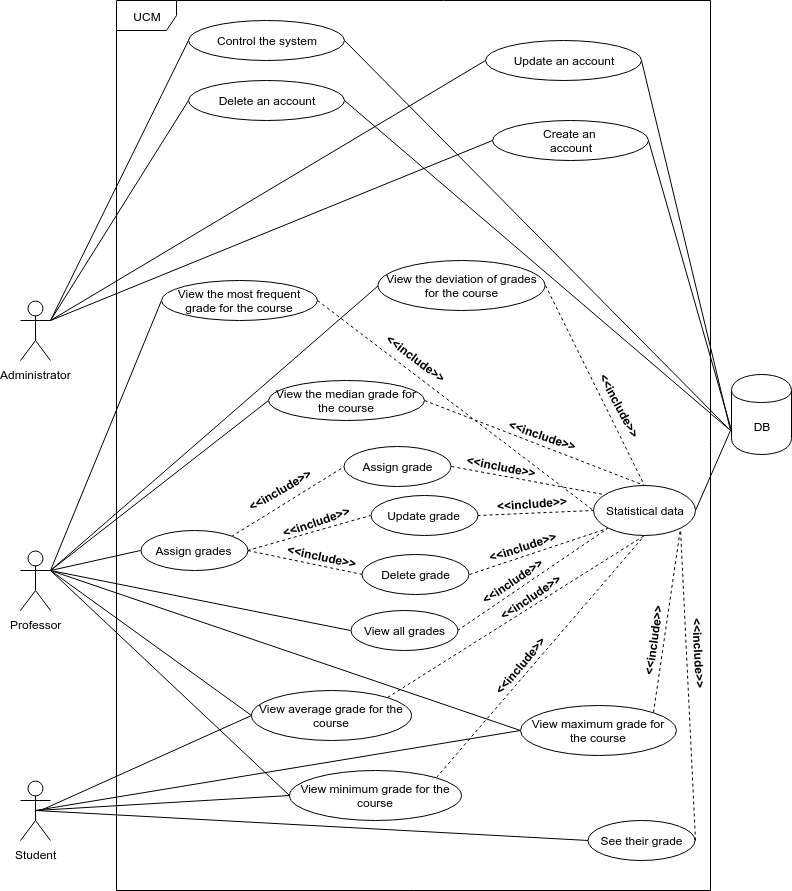
\includegraphics[width=0.89\textwidth]{UCM.png}
\caption{Use case model}
\end{figure}
\newpage
\subsection{Use cases}

\begin{usecase}{Control the system}
    \addrow{Actors}{Administrator, DB}
    \addrow{Precondition}{Administrator has access to the system}
    \addrow{Postcondition}{Administrator has full control of the system}
    \addmulrow{Main scenario (M)}{
        \item Administrator logins to the system
        \item System shows the list of available commands, actions through DB queries
        \item Administrator chooses needed action
        \item System shows the result of the action in log
    }
    \adddoublerow{Extensions (E)}{
        \item[] 1.1. Administrator entered the wrong credentials
        \item[] 1.2. Go to 1
    }
\end{usecase}

\begin{usecase}{Delete an account}
    \addrow{Actors}{Administrator, DB}
    \addrow{Precondition}{Administrator has access to the system}
    \addrow{Postcondition}{Administrator delete an account}
    \addmulrow{Main scenario (M)}{
        \item Administrator logins to the system
        \item System shows the list of available commands, actions through DB queries
        \item Administrator chooses action to delete an account
        \item System shows the list of available accounts
        \item Administrator chooses which account to delete
        \item Administrator deletes an account
        \item System shows the result of the action in log
    }
    \adddoublerow{Extensions (E)}{
        \item[] 1.1. Administrator entered the wrong credentials
        \item[] 1.2. Go to 1
    }
\end{usecase}
\newpage
\begin{usecase}{Create an account}
    \addrow{Actors}{Administrator, DB}
    \addrow{Precondition}{Administrator has access to the system}
    \addrow{Postcondition}{Administrator creates an account}
    \addmulrow{Main scenario (M)}{
        \item Administrator logins to the system
        \item System shows the list of available commands, actions through DB queries
        \item Administrator chooses action to create an account
        \item System shows the form for creating an account
        \item Administrator creates an account credentials
        \item System shows the result of the action in log
    }
    \adddoublerow{Extensions (E)}{
        \item[] 1.1. Administrator entered the wrong credentials
        \item[] 1.2. Go to 1
    }
\end{usecase}

\begin{usecase}{Update an account}
    \addrow{Actors}{Administrator, DB}
    \addrow{Precondition}{Administrator has access to the system}
    \addrow{Postcondition}{Administrator updates an account}
    \addmulrow{Main scenario (M)}{
        \item Administrator logins to the system
        \item System shows the list of available commands, actions through DB queries
        \item Administrator chooses action to update an account
        \item System shows the list of available accounts
        \item Administrator chooses which account to update
        \item Administrator updates an account
        \item System shows the result of the action in log
    }
    \adddoublerow{Extensions (E)}{
        \item[] 1.1. Administrator entered the wrong credentials
        \item[] 1.2. Go to 1
    }
\end{usecase}
\newpage
\begin{usecase}{View the most frequent grade for the course}
    \addrow{Actors}{Professor, DB}
    \addrow{Precondition}{Professor has access to the system}
    \addrow{Postcondition}{Professor views the mode of grades}
    \addmulrow{Main scenario (M)}{
        \item Professor logins to the system
        \item System through statistical data module connects to the DB
        \item System shows the list of available courses
        \item Professor chooses the course to view
        \item System shows the statistics of the course
        \item Professor views the mode of course
    }
    \adddoublerow{Extensions (E)}{
        \item[] 1.1. Professor entered the wrong credentials
        \item[] 1.2. Go to 1
    }
\end{usecase}

\begin{usecase}{View the deviation of grades for the course}
    \addrow{Actors}{Professor, DB}
    \addrow{Precondition}{Professor has access to the system}
    \addrow{Postcondition}{Professor views the deviation of grades}
    \addmulrow{Main scenario (M)}{
        \item Professor logins to the system
        \item System through statistical data module connects to the DB
        \item System shows the list of available courses
        \item Professor chooses the course to view
        \item System shows the statistics of the course
        \item Professor views the deviation of grades
    }
    \adddoublerow{Extensions (E)}{
        \item[] 1.1. Professor entered the wrong credentials
        \item[] 1.2. Go to 1
    }
\end{usecase}
\newpage
\begin{usecase}{View the median grade for the course}
    \addrow{Actors}{Professor, DB}
    \addrow{Precondition}{Professor has access to the system}
    \addrow{Postcondition}{Professor views the median grade}
    \addmulrow{Main scenario (M)}{
        \item Professor logins to the system
        \item System through statistical data module connects to the DB
        \item System shows the list of available courses
        \item Professor chooses the course to view
        \item System shows the statistics of the course
        \item Professor views the median grade
    }
    \adddoublerow{Extensions (E)}{
        \item[] 1.1. Professor entered the wrong credentials
        \item[] 1.2. Go to 1
    }
\end{usecase}

\begin{usecase}{Delete the grades}
    \addrow{Actors}{Professor, DB}
    \addrow{Precondition}{Professor has access to the system}
    \addrow{Postcondition}{Professor deletes the grades.}
    \addmulrow{Main scenario (M)}{
        \item Professor logins to the system
        \item System through statistical data module connects to the DB
        \item System shows the list of available courses
        \item Professor chooses the desirable course
        \item System shows the list of students with their grades
        \item Professor chooses the student
        \item Professor deletes the grade
    }
    \adddoublerow{Extensions (E)}{
        \item[] 1.1. Professor entered the wrong credentials
        \item[] 1.2. Go to 1
    }
\end{usecase}
\newpage
\begin{usecase}{Assign the grades}
    \addrow{Actors}{Professor, DB}
    \addrow{Precondition}{Professor has access to the system}
    \addrow{Postcondition}{Professor assigns the grades.}
    \addmulrow{Main scenario (M)}{
        \item Professor logins to the system
        \item System through statistical data module connects to the DB
        \item System shows the list of available courses
        \item Professor chooses the desirable course
        \item System shows the list of students with their grades
        \item Professor chooses the student
        \item Professor assigns the grade
    }
    \adddoublerow{Extensions (E)}{
        \item[] 1.1. Professor entered the wrong credentials
        \item[] 1.2. Go to 1
    }
\end{usecase}

\begin{usecase}{Update the grades}
    \addrow{Actors}{Professor, DB}
    \addrow{Precondition}{Professor has access to the system}
    \addrow{Postcondition}{Professor updates the grades.}
    \addmulrow{Main scenario (M)}{
        \item Professor logins to the system
        \item System through statistical data module connects to the DB
        \item System shows the list of available courses
        \item Professor chooses the desirable course
        \item System shows the list of students with their grades
        \item Professor chooses the student
        \item Professor updates the grade
    }
    \adddoublerow{Extensions (E)}{
        \item[] 1.1. Professor entered the wrong credentials
        \item[] 1.2. Go to 1
    }
\end{usecase}
\newpage
\begin{usecase}{View all grades}
    \addrow{Actors}{Professor, DB}
    \addrow{Precondition}{Professor has access to the system}
    \addrow{Postcondition}{Professor views the all grades.}
    \addmulrow{Main scenario (M)}{
        \item Professor logins to the system
        \item System through statistical data module connects to the DB
        \item System shows the list of available courses
        \item Professor chooses the desirable course
        \item System shows the list of students with their grades
    }
    \adddoublerow{Extensions (E)}{
        \item[] 1.1. Professor entered the wrong credentials
        \item[] 1.2. Go to 1
    }
\end{usecase}

\begin{usecase}{View average grade for the course}
    \addrow{Actors}{Professor, Student, DB}
    \addrow{Precondition}{Professor has access to the system. Student has access to the system}
    \addrow{Postcondition}{Professor views average grade. Student views average grade.}
    \addmulrow{Main scenario (M)}{
        \item Professor or Student logins to the system
        \item System through statistical data module connects to the DB
        \item System shows the list of available courses for the user (Professor or Student)
        \item Professor or Student chooses the desirable course
        \item System shows the average grade for the course
    }
    \adddoublerow{Extensions (E)}{
        \item[] 1.1. Professor or Student entered the wrong credentials
        \item[] 1.2. Go to 1
    }
\end{usecase}
\newpage
\begin{usecase}{View minimum grade for the course}
    \addrow{Actors}{Professor, Student, DB}
    \addrow{Precondition}{Professor has access to the system. Student has access to the system}
    \addrow{Postcondition}{Professor views minimum grade. Student views minimum grade.}
    \addmulrow{Main scenario (M)}{
        \item Professor or Student logins to the system
        \item System through statistical data module connects to the DB
        \item System shows the list of available courses for the user (Professor or Student)
        \item Professor or Student chooses the desirable course
        \item System shows the minimum grade for the course
    }
    \adddoublerow{Extensions (E)}{
        \item[] 1.1. Professor or Student entered the wrong credentials
        \item[] 1.2. Go to 1
    }
\end{usecase}

\begin{usecase}{View maximum grade for the course}
    \addrow{Actors}{Professor, Student, DB}
    \addrow{Precondition}{Professor has access to the system. Student has access to the system}
    \addrow{Postcondition}{Professor views maximum grade. Student views maximum grade.}
    \addmulrow{Main scenario (M)}{
        \item Professor or Student logins to the system
        \item System through statistical data module connects to the DB
        \item System shows the list of available courses for the user (Professor or Student)
        \item Professor or Student chooses the desirable course
        \item System shows the maximum grade for the course
    }
    \adddoublerow{Extensions (E)}{
        \item[] 1.1. Professor or Student entered the wrong credentials
        \item[] 1.2. Go to 1
    }
\end{usecase}
\newpage
\begin{usecase}{View personal grade for the course}
    \addrow{Actors}{Student, DB}
    \addrow{Precondition}{Student has access to the system}
    \addrow{Postcondition}{Student views their grade.}
    \addmulrow{Main scenario (M)}{
        \item Student logins to the system
        \item System through statistical data module connects to the DB
        \item System shows the list of available courses for the Student
        \item Student chooses the desirable course
        \item System shows the Student's grade for the course
    }
    \adddoublerow{Extensions (E)}{
        \item[] 1.1. Student entered the wrong credentials
        \item[] 1.2. Go to 1
    }
\end{usecase}
%-----------------------------------------------------------------
\section{Part - Estimates of effort}
\subsection{UCP}
The \textbf{UCP} is effort estimation approach. To calculate effort there are number of needed equations: \textbf{UUCP} (Unadjusted Use Case Points), \textbf{TCF} (Technical Complexity Factor), \textbf{ECF} (Environment Complexity Factor). \\
\begin{equation}
    \textbf{UCP} = \textbf{UUCP} \times \textbf{TCF} \times \textbf{ECF}
\end{equation}\\

The \textbf{UUCP} based on the sum of \textbf{UAW} (Unadjusted Actor Weight)
and \textbf{UUCW} (Unadjusted Use Case Weight).\\
\begin{equation}
    \textbf{UUCP} = \textbf{UAW} + \textbf{UUCW}
\end{equation}\\

The \textbf{UAW} based on the aggregated complexity of all the actors in all the use cases.
\begin{equation}
    \textbf{UAW} = \sum^{}_{}{Actors * Weight}
\end{equation}\\
\begin{table}[h]
\centering
\caption{The classification of actors and their associated weights in the UCP approach.}
\begin{tabular}{|l|l|l|}
\hline
\textbf{Actor type} & \textbf{Description} & \textbf{Weight} \\ \hline
A1                  & Simple actor         & 1               \\ \hline
A2                  & Average actor        & 2               \\ \hline
A3                  & Complex actor        & 3               \\ \hline
\end{tabular}
\end{table}
Based on the \textbf{UCM} we have 3 complex actors and 1 simple, then:
\begin{equation}
    \textbf{UAW} = 1\times3 + 1\times3 + 1\times3 + 1\times1
\end{equation}
\begin{equation}
    \textbf{UAW} = 9
\end{equation}\\

the \textbf{UUCW} is based on the total number of steps contained in all the use case scenarios.
\begin{equation}
    \textbf{UUCW} = \sum^{}_{}{UseCase * Weight}
\end{equation}\\
\begin{table}[h]
\centering
\caption{shows that there are 3 types of use cases, each assigned a weight. }
\begin{tabular}{|l|l|l|}
\hline
\textbf{Use Case Type} & \textbf{Description} & \textbf{Weight} \\ \hline
UC1                    & Simple Use Case      & 5               \\ \hline
UC2                    & Average Use Case     & 10              \\ \hline
UC3                    & Complex Use Case     & 15              \\ \hline
\end{tabular}
\end{table}
Based on the \textbf{UCM} we have complex use cases, average use cases and simple usecases, then:
\begin{equation}
    \textbf{UUCW} = 15 \times 5
\end{equation}
\begin{equation}
    \textbf{UUCW} = 75
\end{equation}\\

In this case the \textbf{UUCP} is:
\begin{equation}
    \textbf{UUCP} = 9 + 75
\end{equation}
\begin{equation}
    \textbf{UUCP} = 84
\end{equation}\\

The purpose of \textbf{TCF} (Technical complexity factor) is to account for the technical concerns that can impact the software project from its inception to its conclusion, including delivery.
\begin{equation}
    \textbf{TCF} = C1 + \Bigg[C2 \times \sum^{13}_{i=1}{(W_{Ti} \times F_{i})\Bigg]} 
\end{equation}\\
Where $C1 = 0.6$, $C2 = 0.01$, $W_{Ti}$ is the Technical Complexity Factor Weight, and $F_{i}$ is the Perceived Impact Factor corresponding to each Technical Complexity Factor. 

\begin{table}[h]
\centering
\caption{The Technical Complexity Factors in the UCP approach.}
\begin{tabular}{|l|l|l|l|}
\hline
\multicolumn{1}{|c|}{\textbf{TCF Type}} & \multicolumn{1}{c|}{\textbf{Description}} & \multicolumn{1}{c|}{\textbf{Weight}} & \multicolumn{1}{c|}{\textbf{Factor}} \\ \hline
T1 & Distributed System & 2 & 0 \\ \hline
T2 & Performance & 1 & 5 \\ \hline
T3 & End User Efficiency & 1 & 4 \\ \hline
T4 & Complex Internal Processing & 1 & 3 \\ \hline
T5 & Reusability & 1 & 5 \\ \hline
T6 & Easy to Install & 0.5 & 4 \\ \hline
T7 & Easy to Use & 0.5 & 5 \\ \hline
T8 & Portability & 2 & 5 \\ \hline
T9 & Easy to Change & 1 & 5 \\ \hline
T10 & Concurrency & 1 & 4 \\ \hline
T11 & Special Security Features & 1 & 0 \\ \hline
T12 & Provides Direct Access for Third Parties & 1 & 0 \\ \hline
T13 & Special User Training Facilities are Required & 1 & 0 \\ \hline
\end{tabular}
\end{table}
In this case the \textbf{TCF} is:
\begin{equation}
    \textbf{TCF} =  0.6 + \Big[0.01 \times(2\times0+1\times5+1\times4+1\times3+1\times5+0.5\times4+0.5\times5+2\times5+1\times5+1\times4+1\times0+1\times0+1\times0)\Big]
\end{equation}
\begin{equation}
    \textbf{TCF} =  1.005
\end{equation}\\
\newpage
The purpose of \textbf{ECF} is to account for the development team's personal traits, including experience.
\begin{equation}
    \textbf{ECF} = C1 + \Bigg[C2 \times \sum^{8}_{i=1}{(W_{Ei} \times F_{i})\Bigg]} 
\end{equation}\\
Where $C1 = 1.4$, $C2 = - 0.03$, $W_{Ei}$ is the Environmental Complexity Factor Weight, and $F_{i}$ is the Perceived Impact Factor corresponding to each Environmental Complexity Factor.

\begin{table}[h]
\centering
\caption{The Environmental Complexity Factors in the UCP approach.}
\begin{tabular}{|l|l|l|l|}
\hline
\multicolumn{1}{|c|}{\textbf{ECF Type}} & \multicolumn{1}{c|}{\textbf{Description}} & \multicolumn{1}{c|}{\textbf{Weight}} & \multicolumn{1}{c|}{\textbf{Factor}} \\ \hline
E1 & Familiarity with the Use Case Domain & 1.5 & 4 \\ \hline
E2 & Part-Time Workers & -1 & 3 \\ \hline
E3 & Analyst Capability & 0.5 & 3 \\ \hline
E4 & Application Experience & 0.5 & 4 \\ \hline
E5 & Object-Oriented Experience & 1 & 5 \\ \hline
E6 & Motivation & 1 & 5 \\ \hline
E7 & Difficult Programming Language & -1 & 5 \\ \hline
E8 & Stable Requirements & 2 & 5 \\ \hline
\end{tabular}
\end{table}

In this case the \textbf{ECF} is:
\begin{equation}
    \textbf{ECF} =  1.4 + \Big[-0.03 \times(1.5\times4+(-1\times3)+0.5\times3+0.5\times4+1\times5+1\times5+(-1\times5)+2\times5)\Big]
\end{equation}
\begin{equation}
    \textbf{ECF} =  0.755
\end{equation}\\

The \textbf{UCP} is equal:
\begin{equation}
    \textbf{UCP} = 84 \times 1.005 \times 0.755
\end{equation}
\begin{equation}
    \textbf{UCP} = 63.737
\end{equation}\\

Since the team is new, the \textbf{PF} (Productivity Factor) is equal 20.
In this case the Effort Estimate is:
\begin{equation}
    \textbf{Effort Estimate} = \textbf{UCP} \times \textbf{PF}
\end{equation}
\begin{equation}
    \textbf{Effort Estimate} = 63.737 \times 20
\end{equation}
\begin{equation}
    \textbf{Effort Estimate} = 1274.74 \quad \textrm{person-hours} \quad
\end{equation}\\

Therefore, the estimated effort of the project by using UCP method is \textbf{1275} person-hours.

\subsection{COCOMO 81}
hello world
\subsection{Difference in estimates using UCP and COCOMO 81}
hello world

%-----------------------------------------------------------------
\section{Part - Implementation}
\subsection{Code listings}
The code listing of implemented functions.
\subsubsection{Min function}

\begin{lstlisting}[language=R]
min <- function(array){
  res <- 9999999999999999
  for(elem in array){
    if(elem < res){
      res <- elem
    }
  }
  return(res)
}
\end{lstlisting}

\subsubsection{Max function}

\begin{lstlisting}[language=R]
max <- function(array){
  res <- -9999999999999999
  for(elem in array){
    if(elem > res){
      res <- elem
    }
  }
  return(res)
}
\end{lstlisting}
\subsection{Testing}

%-----------------------------------------------------------------
\section{Part - Cyclomatic complexity}

%-----------------------------------------------------------------
\section{Part - Object-oriented metrics}

%-----------------------------------------------------------------
\section{Part - SLOC}

%-----------------------------------------------------------------
\section{{Part - Correlations}}

%-----------------------------------------------------------------
%Don't delete below
\bibliography{ref}{}
\bibliographystyle{plain}
\end{document}               % End of document.